
\chapter{Basic concepts in the acquisition of medical images}

\section{Energy-tissue interaction}
\begin{itemize}
\item With the exception of \popup{nuclear medicine}{In nuclear
    medicine imaging, radioactive substances are injected or ingested,
    and it is the physiological interactions of the agent that give
    rise to the information in the images.}, all medical imaging
  techniques require that the energy used to penetrate the body's
  tissues also \popup{interacts}{If energy were to pass through the
    body and not experience some type of interaction (e.g., absorption
    or scattering), then the detected energy would not contain any
    useful information regarding the internal anatomy, and thus it
    would not be possible to construct an image of the anatomy using
    that information.} with them \cite{bushberg2011essential} (see
  Figure~\ref{fig:X-rays}).
\end{itemize}
\vspace{-0ex}
\begin{figure}[!h]
  \centering
  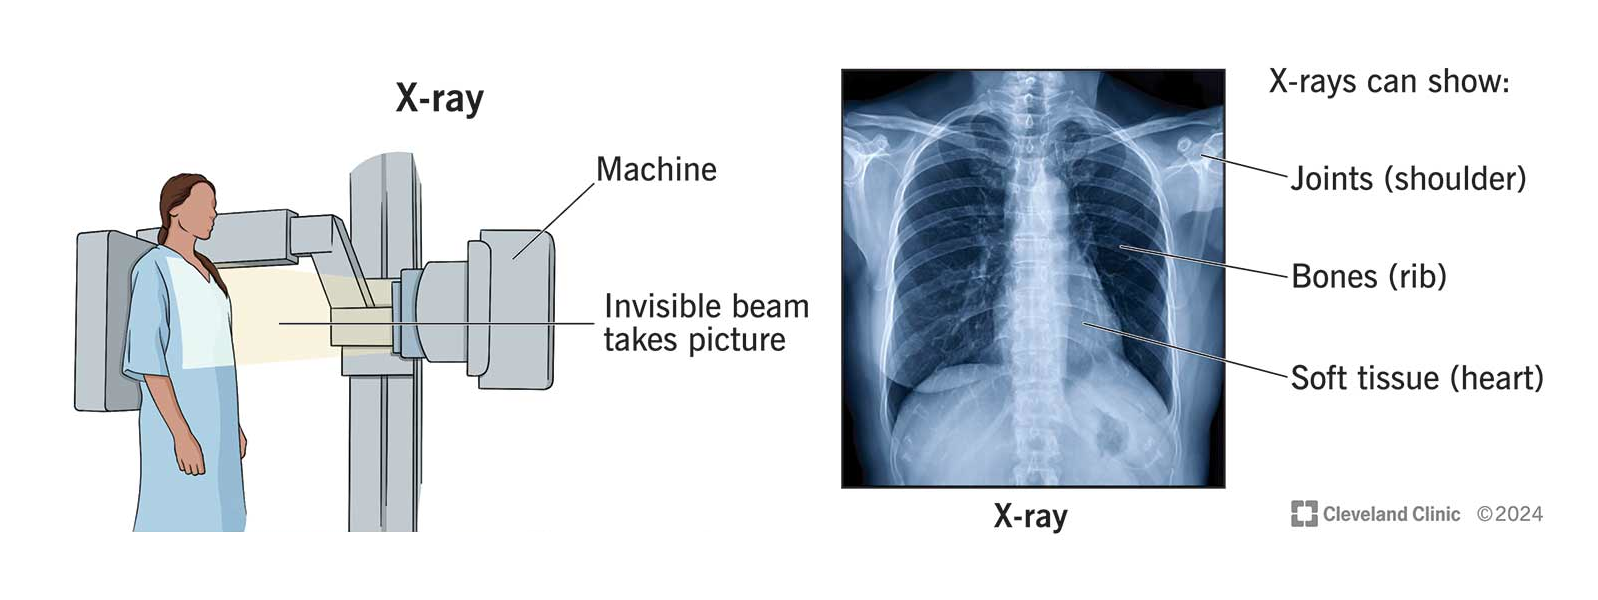
\includegraphics[width=12cm]{X-rays}
  \caption{X-rays machine taking an X-rays image from a
    patient \cite{CC2025Xray}.\label{fig:X-rays}}
\end{figure}

\section{Image quality VS patient safety}
\begin{itemize}
\item The power, energy and time required to acquiring medical images
  require a \popup{compromise}{Better x-ray images can be made when
    the radiation dose to the patient is high, better magnetic
    resonance images can be made when the image acquisition time is
    long, and better ultrasound images result when the ultrasound
    power levels are large.} between patient safety and image quality
  \cite{bushberg2011essential} (see
  Figure~\ref{fig:quality_vs_radiation}).
\end{itemize}
\vspace{-0ex}
\begin{figure}[!h]
  \centering
  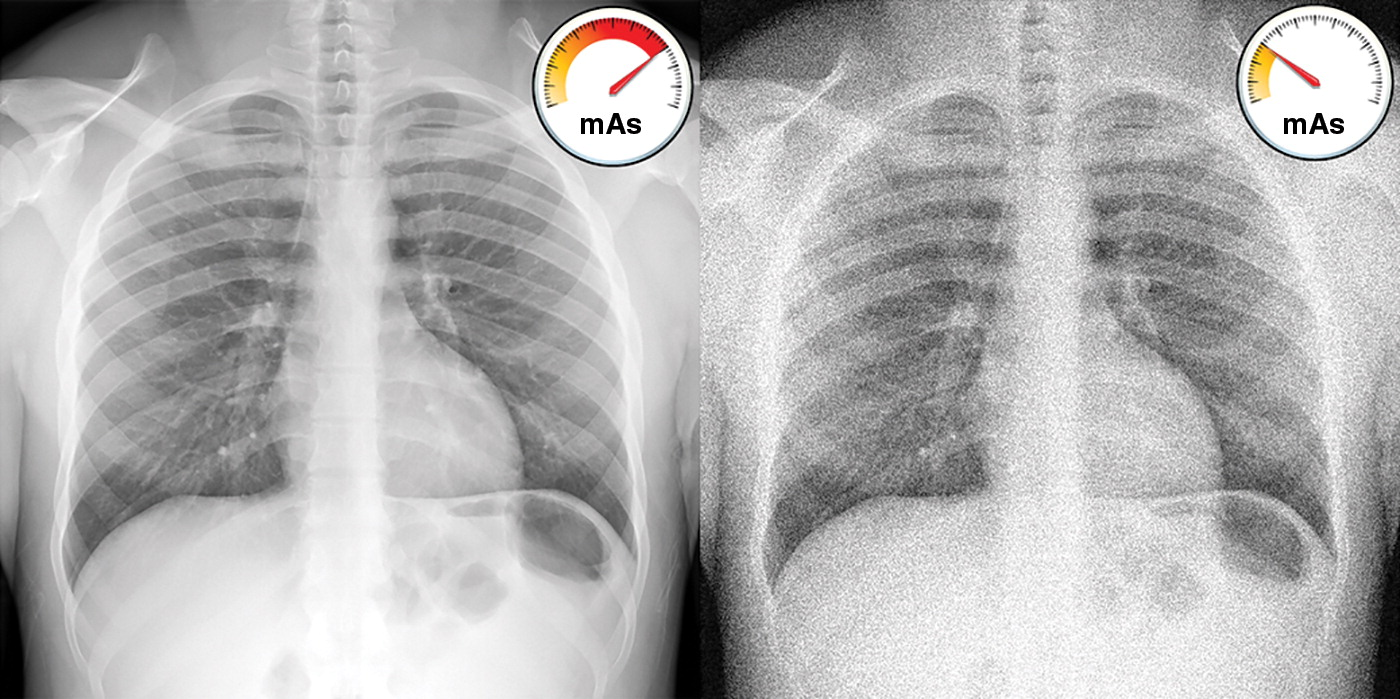
\includegraphics[width=8cm]{X-rays__quality_vs_radiation}
  \caption{Quality VS radiation dose (measured in milliampere-second,
    i.e., the electric charge provided to the X-rays
    machine))
    \cite{huda2015radiographic}.\label{fig:quality_vs_radiation}}
\end{figure}

\section{Digital media}
\begin{itemize}
\item Most modern medical imaging systems are digital.
\item Convert \popup{continuous}{A continuous signal it defined at any
    instant of time or space.} (\popup{analog}{An analog signal can
    take an infinite number of values (for example, the amount of
    water that we can put into a glass.)}) signals from detectors into
  digital data. This conversion, known as digitization, involves two
  main steps:
  \begin{enumerate}
  \item \textbf{Sampling}: Selection specific points in time (or
    space) for conversion.
  \item \textbf{Quantization}: Conversion of each analogue sample into a
    digital number.
  \end{enumerate}
\end{itemize}

\section{Noise}
\begin{itemize}
\item The processes by which radiation is emitted and interacts with
  matter are inherently random, making all radiation measurements,
  including medical imaging, subject to random error
  \cite{bushberg2011essential}.
\end{itemize}

\section{Quantization noise}
\begin{itemize}
\item A \popup{band-limited signal}{A band-limited signal requires
    only a finite interval of frequencies.} can be sampled without
  loss of information. However, quantization always loss some kind of
  information, generating the so called \emph{quantization noise}.
\item To reduce the quantization noise, \popup{the
number of bits/sample must be high enough}{For instance, X-ray CT
  requires 12 bits per pixel due to its high contrast resolution,
  whereas ultrasound typically uses 8 bits due to its limited contrast
  resolution.} \cite{bushberg2011essential}.
\item Usually, quantization \popup{replaces \emph{real}
    noise}{Physically, it is impossible to obtain a perfect digital
    signal (without any kind of noise) because the acquisition systems
    are intrinsically noisy.} by quantization noise, and therefore,
  the impact of using a finite number of bits is, in some way, limited
  (or at least, controlled).
\end{itemize}
